%
% $File: report.tex
% $Date: Sun Dec 15 15:33:10 2013 +0800
%

\documentclass{article}
\usepackage{fontspec}
\usepackage{zhspacing,url,amsmath,amssymb,verbatim}
\usepackage{pdfpages}
\zhspacing
\usepackage{listings}
\usepackage[hyperfootnotes=false,colorlinks,linkcolor=blue,anchorcolor=blue,citecolor=blue]{hyperref}
\usepackage[backend=biber]{biblatex}
\usepackage{graphicx}
\usepackage{minted}
\usepackage{subfigure}
\usepackage{indentfirst}
\usepackage{cases}
\usepackage{environ}
\usepackage{array}
\usepackage[top=1in, bottom=1in, left=1.25in, right=1.25in]{geometry}
\usepackage{caption}
%\usepackage{tikz}
%\usepackage{dot2texi}

% $File: mint-defs.tex
% $Date: Thu Sep 26 22:11:33 2013 +0800
% $Author: Xinyu Zhou <zxytim@gmail.com>

\newcommand{\inputmintedConfigured}[3][]{\inputminted[fontsize=\footnotesize,
	label=#3,linenos,frame=lines,framesep=0.8em,tabsize=4,#1]{#2}{#3}}

\newcommand{\txtsrc}[2][]{\inputmintedConfigured[#1]{text}{#2}}
\newcommand{\txtsrcpart}[4][]{\txtsrc[firstline=#3,firstnumber=#3,lastline=#4,#1]{#2}}

\newcommand{\cppsrc}[2][]{\inputmintedConfigured[#1]{cpp}{#2}}
\newcommand{\cppsrcpart}[4][]{\cppsrc[firstline=#3,firstnumber=#3,lastline=#4,#1]{#2}}

\newcommand{\javasrc}[2][]{\inputmintedConfigured[#1]{java}{#2}}
\newcommand{\javasrcpart}[4][]{\javasrc[firstline=#3,firstnumber=#3,lastline=#4,#1]{#2}}

\newcommand{\matlabsrc}[2][]{\inputmintedConfigured[#1]{matlab}{#2}}
\newcommand{\matlabsrcpart}[4][]{\matlabsrc[firstline=#3,firstnumber=#3,lastline=#4,#1]{#2}}

%\usepackage[T1]{fontenc}
\usepackage{lmodern}
\usepackage{amssymb,amsmath}
\usepackage{ifxetex,ifluatex}
\usepackage{fixltx2e} % provides \textsubscript
% use upquote if available, for straight quotes in verbatim environments
\IfFileExists{upquote.sty}{\usepackage{upquote}}{}
\ifnum 0\ifxetex 1\fi\ifluatex 1\fi=0 % if pdftex
  \usepackage[utf8]{inputenc}
\else % if luatex or xelatex
  \usepackage{fontspec}
  % commented by Xinyu Zhou
  \ifxetex
    \usepackage{xltxtra,xunicode}
  \fi
  \defaultfontfeatures{Mapping=tex-text,Scale=MatchLowercase}
  \newcommand{\euro}{€}
\fi
% use microtype if available
\IfFileExists{microtype.sty}{\usepackage{microtype}}{}
\usepackage{color}
\usepackage{fancyvrb}
\newcommand{\VerbBar}{|}
\DefineShortVerb[commandchars=\\\{\}]{\|}
\DefineVerbatimEnvironment{Highlighting}{Verbatim}{commandchars=\\\{\}}
% Add ',fontsize=\small' for more characters per line
\newenvironment{Shaded}{}{}
\newcommand{\KeywordTok}[1]{\textcolor[rgb]{0.00,0.44,0.13}{\textbf{{#1}}}}
\newcommand{\DataTypeTok}[1]{\textcolor[rgb]{0.56,0.13,0.00}{{#1}}}
\newcommand{\DecValTok}[1]{\textcolor[rgb]{0.25,0.63,0.44}{{#1}}}
\newcommand{\BaseNTok}[1]{\textcolor[rgb]{0.25,0.63,0.44}{{#1}}}
\newcommand{\FloatTok}[1]{\textcolor[rgb]{0.25,0.63,0.44}{{#1}}}
\newcommand{\CharTok}[1]{\textcolor[rgb]{0.25,0.44,0.63}{{#1}}}
\newcommand{\StringTok}[1]{\textcolor[rgb]{0.25,0.44,0.63}{{#1}}}
\newcommand{\CommentTok}[1]{\textcolor[rgb]{0.38,0.63,0.69}{\textit{{#1}}}}
\newcommand{\OtherTok}[1]{\textcolor[rgb]{0.00,0.44,0.13}{{#1}}}
\newcommand{\AlertTok}[1]{\textcolor[rgb]{1.00,0.00,0.00}{\textbf{{#1}}}}
\newcommand{\FunctionTok}[1]{\textcolor[rgb]{0.02,0.16,0.49}{{#1}}}
\newcommand{\RegionMarkerTok}[1]{{#1}}
\newcommand{\ErrorTok}[1]{\textcolor[rgb]{1.00,0.00,0.00}{\textbf{{#1}}}}
\newcommand{\NormalTok}[1]{{#1}}
% \ifxetex
%   \usepackage[setpagesize=false, % page size defined by xetex
%               unicode=false, % unicode breaks when used with xetex
%               xetex]{hyperref}
% \else
%   \usepackage[unicode=true]{hyperref}
% \fi
\hypersetup{breaklinks=true,
            bookmarks=true,
            pdfauthor={},
            pdftitle={},
            colorlinks=true,
            urlcolor=blue,
            %linkcolor=magenta,
            pdfborder={0 0 0}}
%\urlstyle{same}  % don't use monospace font for urls
\setlength{\parindent}{0pt}
\setlength{\parskip}{6pt plus 2pt minus 1pt}
\setlength{\emergencystretch}{3em}  % prevent overfull lines
%\setcounter{secnumdepth}{0}



\newcommand{\figref}[1]{\hyperref[fig:#1]{Figure\ref*{fig:#1}}}
\newcommand{\tableref}[1]{\hyperref[table:#1]{Table\ref*{table:#1}}}
\newcommand{\centerize}[1]{\begin{center} #1 \end{center}}

\newcommand{\cmd}[1]{{\it #1}}
\newcommand{\ccmd}[1]{\centerize{\cmd{#1}}}

\title{Digital Signal Processing: Speaker Recognition \\ Stage Report}
\author{Xinyu Zhou, Yuxin Wu, and Tiezheng Li\\ Tsinghua University}
\date{}

\bibliography{refs.bib}
\begin{document}

\fontsize{11pt}{1.4em}
\setlength{\baselineskip}{1.6em}
\maketitle


\section{Introduction}
A \textbf{Speaker Recognition} tasks can be classified with respect to different criterion:
Text-dependent or Text-independent, Verification (decide whether the person is he claimed to be) or Identification (decide who the person is by its voice).\cite{SRwiki}

Speech is a kind of complicated signal produced as a result of several transformations occurring at different levels: semantic, linguistic and acoustic.
Differences in these transformations may lead to differences in the acoustic properties of the signals.
The recognizability of speaker can be affected not only by the linguistic message
but also the age, health, emotional state and effort level of the speaker.
Background noise and performance of recording device also interfere
the classification process.

Speaker recognition is an important part of Human-Computer Interaction (HCI).
As the trend of employing wearable computer reveals,
Voice User Interface (VUI) has been a vital part of such computer.
As these devices are particularly small, they are more likely to lose and be stolen.
In these scenarios, speaker recognition is not only a good HCI,
but also a combination of seamless interaction with computer and security guard
when the device is lost.
The need of personal identity validation will become more acute in the future.
Speaker verification may be essential in business telecommunications.
Telephone banking and telephone reservation services will develop rapidly
when secure means of authentication were available.

Also,the identity of a speaker is quite often at issue in court cases.
A crime victim may have heard but not seen the perpetrator,
but claim to recognize the perpetrator as someone whose voice was previously familiar;
or there may be recordings of a criminal whose identity is unknown.
Speaker recognition technique may bring a reliable scientific determination.

Furthermore, these techniques can be used in environment which demands high security.
It can be combined with other biological metrics to form a multi-modal authentication system.

In this task, our goal is to build a proof-of-concept text-dependent speaker recognition system with GUI support.
Hopefully, we would like to extend its ability to a text-independent speaker recognition system.

\section{Approach}
	In this section we will present our aproach to tackle the speaker recognition problem.
	There're two steps in a complete speaker recognition system: enrollment and recognition.

\subsection{Erollment}
	\label{sec:approach_enrollment}
	An utterance of a user is collected during enrollment procedure.
	Further processing of the utterance follows following steps:
	\begin{enumerate}
		\item \textbf{VAD} \\
            Signals must be first filtered to rule out the silence part, otherwise the
            training might be seriously biased. Therefore \textbf{Voice Activity Detection} must
            be first performed.
			An observation found is that, the corpus provided is nearly noise-free.
            Therefore we use a simple energy-based approach
			to remove the silence part, by simply remove the frames that the average
            energy is below 0.01 times the average energy of the whole utterance.

            This energy-based method is found to work well on database, but not
            on GUI. We use LTSD(Long-Term Spectral Divergence) \cite{ltsd1} algorithm on GUI, as well as
            noise reduction technique from SOX\cite{sox} to gain better result.

		\item \textbf{MFCC and LPC Features} \\ We extract
          \textbf{Mel-frequency cepstral coefficients} and \textbf{Linear Predictive
			Coding} features using following parameter are found to be
			optimal, according to our experiments in \secref{result}:

			\begin{itemize}
				\item Common parameters:
					\begin{itemize}
						\item Frame size: 32ms
						\item Frame shift: 16ms
						\item Preemphasis coefficient: 0.95
					\end{itemize}
				\item MFCC parameters:
					\begin{itemize}
						\item number of cepstral coefficient: 15
						\item number of filter banks: 55
						\item maximal frequency of the filter bank: 6000
					\end{itemize}
				\item LPC Parameters:
					\begin{itemize}
						\item number of coefficient: 23
					\end{itemize}
			\end{itemize}

			and then concatenate the two feature vectors of the same frame forming
			a larger feature vector of 15 + 23 = 38 dimension.

		\item \textbf{GMM}

			We use \textbf{Gaussian Mixture Model} modeling a speaker. Some improvements made:
			\begin{itemize}
				\item Performance: \\
					We investigate the effect of initialization of GMM during
					training. We implemented GMM with
					K-meansII\cite{bahmani2012scalable}, which is an improved
					version of K-means++\cite{arthur2007k} to initialize the
					mean vector of GMM. Results shows improvements compared
					to GMM provided by \textbf{scikit-learn\cite{scikit-learn}}.
				\item Efficiency:
					\begin{itemize}
						\item We provide a parallel version of GMM, especially
							optimized to train large Universal Background Model(UBM).
						\item We further improve efficiency by utilizing
							SSE instruction in computing exponential function
							using polynomial approximation. This can speed up
							the training procedure by a factor of two.
					\end{itemize}
                \end{itemize}

		\item \textbf{UBM}

			As we are providing continuous speech close-set diarization function in
			GUI, we adopt \textbf{Universal Background Model} as imposter model,
			and use likelihood ratio test to make reject
			decisions.\cite{reynolds2000speaker}

			When using conversation mode in GUI (will be present later),
			GMM model of each user is adapted from a pre-trained UBM
			using method described in \cite{reynolds2000speaker}.

		\item \textbf{CRBM}

          \textbf{Restricted Boltzmann Machine} is generative stochastic
			two-layer neural network that can learn a probability distribution
			over its set of binary inputs\cite{rbm_wiki}.  \textbf{Continuous
			restricted Boltzmann Machine(CRBM)}\cite{chen2003continuous} extends
			its ability to real-valued inputs.  RBM has a ability to, given an
			input(visible layer), reconstruct a visible layer that is similar
			to the input.  \figref{crbm} illustrate original MFCC data and the
			sampled output of
			reconstructed data from CRBM.


		\item \textbf{JFA}:

          \textbf{Joint Factor Analysis} \cite{jfa2,jfa-se} was generally considered to perform better than other method
          in the task of Speaker Recognition, by modeling different types of variabilities in the training data, including session variability and
          speaker variability.

          Therefore, we use a simpler algorithm presented in \cite{jfa-study} to train the JFA model.
          However, the result shows that JFA does not seem to outperform GMM.
          We suspected that the training of a JFA model needs more data than
          we provided, since JFA needs data from various source to account for different types of variabilities.
          To get a higher accuracy in JFA, We might need to add extra data for training.
	\end{enumerate}

\subsection{Recognition}
	Recognition procedure follows steps below:
	\begin{enumerate}
		\item Record a short utterance of the speaker (typically less than 5 seconds)

		\item Preprocess the utterance using first two steps described in
			\secref{approach_enrollment}, e.g, VAD, MFCC and LPC feature extraction.

		\item Compute the `score' of each person enrolled, and adopt person
			corresponding the model which gives highest score to be the
			recognition result.

			A typical form of score is log-likelihood (or energy in RBM case).
	\end{enumerate}

\section{Performance}
\label{sec:result}
We have tested our approaches under various parameters, based on a corpus provided by teacher Xu.
For detailed description of the corpus, please see former report.

All the tests in this section have been conducted serval times
(depending on computation cost, vary from 10 to 30)
with random selected training and testing speakers.
The average over these tests are considered as confidential result.

%\subsection{Efficiency Test of our GMM}
%We have extensively examined the efficiency of our implementation of GMM
%compared to scikit-learn version. Test is conducted using real MFCC data with
%13 dimensions. We consider the scenario when training a UBM with 256 mixtures.
%We examine the time used for ten iteration.  For comparable results, we diabled
%the K-means initialization process of both scikit-learn GMM implementation and
%ours.  Time used for ten iterations under different data size and concurrency
%is recorded.

%From \figref{gmm_efficiency}, we can immediately infer that our method
%is much-much more efficient than the widely used version of GMM provided
%by scikit-learn when the data size grows sufficiently large.

%We shall analyze in two aspect:
%\begin{itemize}
	%\item No concurrency
		%\begin{itemize}
			%\item When the number of MFCC features is below 6000, which is a typical
				%number of features generated by 60 seconds utterances (1ms frame shift),
				%our method is slightly slower; but this is trivial since
				%1 minute utterance is too small.
			%\item When the number of MFCC features grows sufficiently large, our method
				%shows great improvement. When training 512,000 features, our method
				%is 5 times faster than comparing method.
		%\end{itemize}
	%\item With concurrency \\
		%Our method shows considerable concurrency scalability that the running time
		%is approximately lineary to the number of cores using.

		%When using 8-cores, our method is \textbf{$19$ times} faster than comparing
		%method.
%\end{itemize}


\subsection{Change in MFCC Parameters}
\begin{enumerate}
    \item Different Number of Cepstrums

      \item Different Number of Filterbanks

        \item Different Size of Frame
\end{enumerate}

\subsection{Change in LPC Parameters}
\begin{enumerate}
    \item Different Number of Coefficient

        \item Different Size of Frame
\end{enumerate}

\subsection{Change in GMM Components}

We examined our GMM compared to GMM from scikit-learn.
Test is conducted on 30-speaker corpus, 30 seconds training utterance
and 100 random sampled 5 seconds test utterance for each speaker.

As \figref{mixture} illustrates, when number of mixtures is small,
our GMM outperforms scikit-learn version by $10\%$, which indicates our
GMM models the distribution more accurately. The maximum accuracy
happens when the number of mixtures is around 32, reaching $0.965$. As
the number of mixtures increases, the decrease in accuracy

\subsection{Performance with Well-Tuned Parameters}

An apparent trade-off in speaker recognition task is the number of speakers
enrolled and the accuracy on recognization.
Also, the duration of signal for enrollment and test can have significant effect on the accuracy.
We've conducted test using well-tuned parameters for feature extraction and GMM, on dataset with
various number of people and with various test duration.

The configurations of this experiment is as followed:
\begin{itemize}
  \item MFCC: frame size is $32 ms $, 19 cepstrums, 55 filterbanks
  \item LPC: frame size is $32 ms $, 15 coefficients
  \item GMM from scikit-learn, number of mixtures is 32
  \item 20s utterance for enrollment
  \item 50 sampled test utterance for each user
\end{itemize}


Scrunitizing \figref{nspk_enrolled} we would see that, our GMM performs better than
scikit GMM in general. When number of speakers is small, due to the random
selection, the variance of the tests is significantly high, as we can see from the curve fluctuants.
When number of speakers increases, it is clear that the
accuracy of our GMM is above scikit version. As the more speaker, the more
difficult the recognition task will be, this result suggests that our
optimization on GMM takes effect.



\section{GUI}
\label{sec:gui}
The GUI contains following tabs:
\begin{itemize}
  \item \textbf{Enrollment} \\

    \begin{figure}[H]
      \centering
      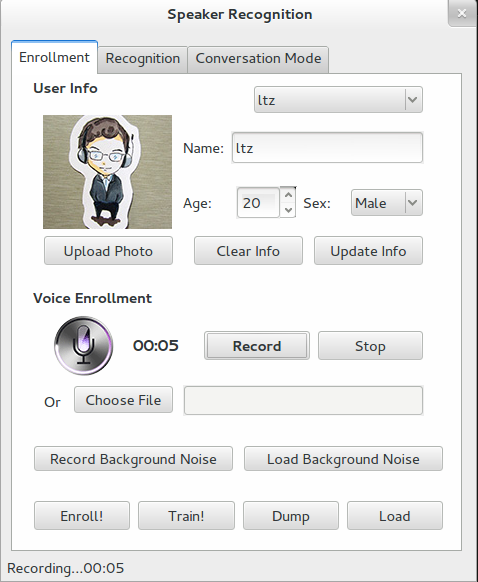
\includegraphics[width=0.8\textwidth]{img/enrollment.png}
    \end{figure}

    A new user may start his or her first step by clicking the
    tab Enrollment. New users could provide personal information
    such as name, sex, and age. then upload personal avatar to
    build up their own data. Experienced users can choose from
    the userlist and update their infomation.

    Next the user needs to provide a piece of utterance for
    the enrollment and training process.

    There are two ways to enroll a user:
    \begin{itemize}
      \item \textbf{Enroll by Recording}
        Click Record and start talking while click Stop to stop
        and save.There is no limit of the content of the utterance,
        whileit is highly recommended that the user speaks long enough
        to provide sufficient message for the enrollment.

      \item \textbf{Enroll from Wav Files}
        User can upload a pre-recorded voice of a speaker.(*.wav recommended)
        The systemaccepts the voice given and the enrollment of a speaker is done.
    \end{itemize}

    The user can train, dump or load his/her voice features after enrollment.

  \item \textbf{Recognition of a user} \\
    \begin{figure}[H]
      \centering
      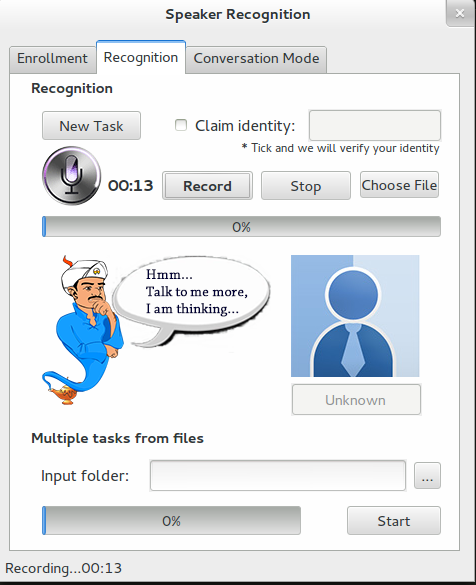
\includegraphics[width=0.8\textwidth]{img/recognition.png}
    \end{figure}

    A enrolled user present or record a piece of utterance,
    the system tells who the person is and show user's avatar.
    Recognition of multiple pre-recorded files can be done as well.

  \item \textbf{Conversation Recognition Mode} \\
    \begin{figure}[H]
      \centering
      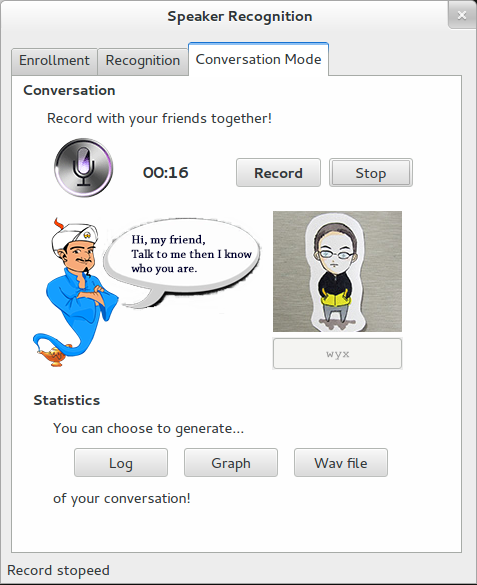
\includegraphics[width=0.8\textwidth]{img/conversation.png}
      \caption{\label{fig:}}
    \end{figure}

    In Conversation Recognition mode, multiple users can have conversations
    together near the microphone. Same recording procedure as above.
    The system will continuously collect voice data, and determine
    who is speaking right now. Current speaker's anvatar will show up
    in screen; otherwise the name will be shown. The conversation
    audio can be downloaded and saved.
    There are some ways to visualize the speaker-distribution in the
    conversation.
    \begin{itemize}
      \item \textbf{Conversation log}
        A detailed log, including start time, stop time,
        current speaker of each period is generated.
      \item \textbf{Conversation flow graph}
        \begin{figure}[H]
          \centering
          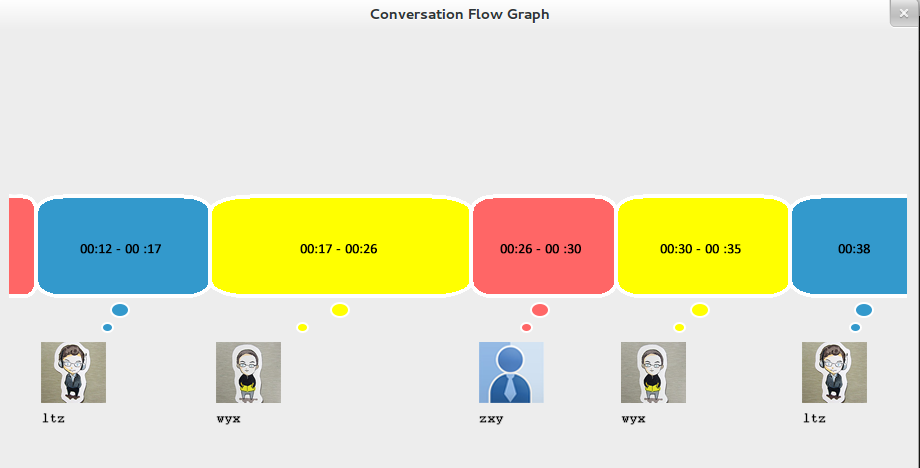
\includegraphics[width=0.8\textwidth]{img/conversationgraph.png}
        \end{figure}

        A timeline of the conversation will be shown by a number of
        talking-clouds joining together, with start time, stop time
        and users' avatars labeled. Different users are presented
        with different colors.The timeline will flow to the left dynamically
        just as time elapses. The visualization of the conversation is done
        in this way. This functionality is still under development.
    \end{itemize}

\end{itemize}


\printbibliography

\end{document}

